\subsection{Design}\label{sec:design}
For this project, I used a user-centered design approach, beginning by identifying the characteristics and goals of its target audience. With those users in mind, I determined the tasks the final webpage should support---what kinds of questions it needed to answer, how much context it would provide, and what resources it should include for further exploration. These decisions guided the selection of relevant design principles, which in turn shaped the resulting designs.

\subsubsection{Users}\label{users}
My project is intended for a general audience, not simply for women's advocates within technology. Most viewers will probably have an interest in the topic, as a woman, as someone who cares about technology, or both; but they may not have any exposure to gender diversity statistics within tech. This motivates a narrative thread throughout the page, rather than analytical visualizations presented without comment, both to provide context and to help them interpret the data visualizations.

I used two primary personas to guide my design work:
\begin{itemize}
  \item Gabriella Griffin, 19, undergraduate psychology major
  \item Laurie Woods, 28, web designer/front-end developer
\end{itemize}
Together, they include both casual audiences (Gabriella) and those invested in diversity in tech (Laurie). Details for each persona are included in \autoref{fig:personas}.

\begin{figure}
  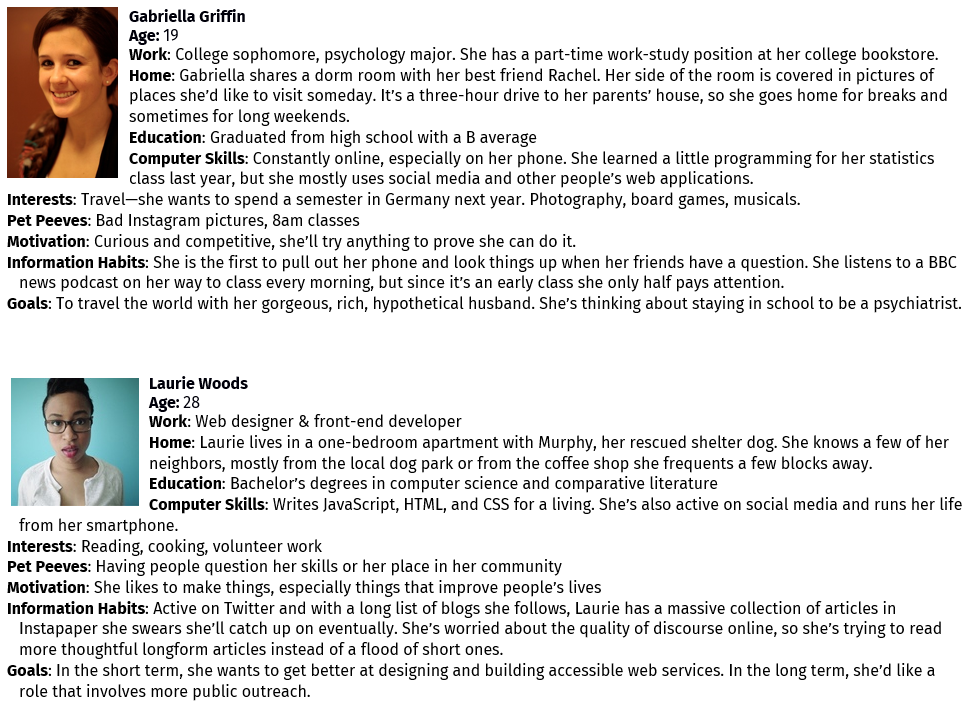
\includegraphics[width=0.9\textwidth]{personas}
  %% TODO: Add profiles %%
  \caption{Primary Personas: Gabriella Griffin \& Laurie Woods}\label{fig:personas}
\end{figure}

\subsubsection{Tasks}\label{tasks}
I do not assume viewers have any prior exposure to diversity statistics or to the tech industry. For users like Gabriella, the primary task the project supports is noticing the gender imbalance at all stages in the tech pipeline. Users like Laurie, who are already aware of the problem, can explore the statistics to see the extent of the problem. The project provides an overview of the data to give this high-level introduction to tech demographics, then presents each stage of the pipeline individually, allowing viewers to explore questions like:

\begin{itemize}
  \item When do women get involved in tech? Is a computer science degree required?
  \item Where does the pipeline leak? Is there a stage when more women seem to drop out?
  \item What kinds of technical careers are open to women? What kinds are still relatively closed?
  \item Does exposing girls to computer science at younger ages lead to more women working in IT\@?
\end{itemize}

The project should also answer questions about the importance of gender diversity in tech and about the interventions used to increase women's participation in IT\@. This includes presenting background information from prior research and providing resources where interested viewers can learn more, from the data used in the visualizations to media coverage to company diversity policies.

To provide high-level context and allow more detailed exploration, I use an ``overview first, details on demand'' strategy. While this is usually used to describe individual data visuallizations, I use it to structure the webpage itself. Viewers see an overview of the pipeline first, to provide a conceptual map of the rest of the project. They are then able to choose a specific section of the pipeline to see more information immediately, or to scroll through the page to view the entire pipeline in chronological order. The detail views are designed for consistency, to facilitate comparison across stages.
